\pdfminorversion=4
\documentclass[aspectratio=169]{beamer}

\mode<presentation>
{
  \usetheme{default}
  \usecolortheme{default}
  \usefonttheme{default}
  \setbeamertemplate{navigation symbols}{}
  \setbeamertemplate{caption}[numbered]
  \setbeamertemplate{footline}[frame number]  % or "page number"
  \setbeamercolor{frametitle}{fg=white}
  \setbeamercolor{footline}{fg=black}
} 

\usepackage[english]{babel}
\usepackage[utf8x]{inputenc}
\usepackage{tikz}
\usepackage{courier}
\usepackage{array}
\usepackage{bold-extra}
\usepackage{minted}
\usepackage[thicklines]{cancel}
\usepackage{fancyvrb}
\usepackage{tabto}

\xdefinecolor{dianablue}{rgb}{0.18,0.24,0.31}
\xdefinecolor{darkblue}{rgb}{0.1,0.1,0.7}
\xdefinecolor{darkgreen}{rgb}{0,0.5,0}
\xdefinecolor{darkgrey}{rgb}{0.35,0.35,0.35}
\xdefinecolor{darkorange}{rgb}{0.8,0.5,0}
\xdefinecolor{darkred}{rgb}{0.7,0,0}
\definecolor{darkgreen}{rgb}{0,0.6,0}
\definecolor{mauve}{rgb}{0.58,0,0.82}

\title[2019-06-19-nyu-as-jimstuff]{``Jim stuff''}
\author{Jim Pivarski}
\institute{Princeton University -- IRIS-HEP}
\date{June 19, 2019}

\usetikzlibrary{shapes.callouts}

\begin{document}

\logo{\pgfputat{\pgfxy(0.11, 7.4)}{\pgfbox[right,base]{\tikz{\filldraw[fill=dianablue, draw=none] (0 cm, 0 cm) rectangle (50 cm, 1 cm);}\mbox{\hspace{-8 cm}\includegraphics[height=1 cm]{princeton-logo-long.png}\hspace{0.1 cm}\raisebox{0.1 cm}{\includegraphics[height=0.8 cm]{iris-hep-logo-long.png}}\hspace{0.1 cm}}}}}

\begin{frame}
  \titlepage
\end{frame}

\logo{\pgfputat{\pgfxy(0.11, 7.4)}{\pgfbox[right,base]{\tikz{\filldraw[fill=dianablue, draw=none] (0 cm, 0 cm) rectangle (50 cm, 1 cm);}\mbox{\hspace{-8 cm}\includegraphics[height=1 cm]{princeton-logo.png}\hspace{0.1 cm}\raisebox{0.1 cm}{\includegraphics[height=0.8 cm]{iris-hep-logo.png}}\hspace{0.1 cm}}}}}

% Uncomment these lines for an automatically generated outline.
%\begin{frame}{Outline}
%  \tableofcontents
%\end{frame}

% START START START START START START START START START START START START START

\begin{frame}{Apologies for any misrepresentation}
\vspace{0.1 cm}
\begin{columns}
\column{1.15\linewidth}
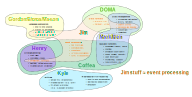
\includegraphics[width=\linewidth]{everybody.pdf}
\end{columns}
\end{frame}

\begin{frame}{Projects and collaborations}
\vspace{0.5 cm}
\begin{columns}
\column{1.15\linewidth}
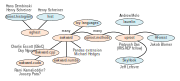
\includegraphics[width=\linewidth]{projects.pdf}
\end{columns}
\end{frame}

\begin{frame}{Year of teaching}
\vspace{0.5 cm}
\large

\begin{itemize}\setlength{\itemsep}{0.25 cm}
\item \textcolor{darkblue}{April 1:}     \tabto{2.3 cm}Software Carpentry at Fermilab (intensity frontier)
\item \textcolor{darkblue}{April 8--10:} \tabto{2.3 cm}PICSciE Numpy course at Princeton (mostly science)
\item \textcolor{darkblue}{May 6:}       \tabto{2.3 cm}Language tools tutorial at ADL workshop (particle physics)
\item \textcolor{darkblue}{May 28--29:}  \tabto{2.3 cm}Scientific Python and columnar analysis HATS (CMS)
\item \textcolor{darkblue}{June 10:}     \tabto{2.3 cm}Software Carpentry at Argonne (U.S.\ ATLAS)
\item \textcolor{darkblue}{July 22--26:} \tabto{2.3 cm}CoDaS-HEP (particle physics)
\end{itemize}

\vspace{0.5 cm}
\begin{itemize}
\item Pratyush Das (IRIS-HEP fellow)
\item Charlie Escott (GSoC)
\item Duy Nguyen (volunteer)
\end{itemize}
\end{frame}


\end{document}
